% Partie : histoire
% Chapitre : théorie des ensembles
% Section : limites

\documentclass[../../../include/open-logic-section]{subfiles}

\begin{document}

\olfileid[fr]{his}{set}{limits}

\olsection{Définition rigoureuse des limites}

De nos jours, la solution habituelle au problème précédent consiste
à se passer des infinitésimaux. Voici comment.

Nous avons vu que, lorsque $\beta$ diminue, les approximations de la
pente s'améliorent. Quand $\beta$ se rapproche autant que l'on veut
de~$0$, le quotient différentiel tend vers la pente recherchée.\footnote{
Correction mathématique de l'édition française : la source anglaise
fait varier $f'(c)$ avec $\beta$, alors que $f'(c)$ désigne une valeur
fixe. C'est le quotient différentiel qui varie.} Au lieu de nous
demander ce qui se passe \emph{pour} $\beta = 0$, il suffit donc
d'étudier la \emph{tendance} du quotient différentiel lorsque
$\beta$ s'approche de~$0$.

Formulé de manière générale, le problème consiste à donner un sens
à un énoncé de cette forme :
\begin{center}
Lorsque $x$ s'approche de $c$, $g(x)$ tend vers $\ell$.
\end{center}
Nous pouvons l'écrire plus brièvement ainsi :
\[
\lim_{x \rightarrow c}g(x) = \ell.
\]
Au XIXe siècle, Weierstrass, s'appuyant sur les travaux antérieurs de
Cauchy, donna de cette expression une définition parfaitement
rigoureuse. L'idée est que l'on peut rendre $g(x)$ aussi proche que
l'on veut de~$\ell$ en choisissant $x$ suffisamment proche de~$c$.
Plus précisément, nous posons que
$\lim_{x \rightarrow c} g(x) = \ell$ signifie :\footnote{
Convention de l'édition française : la limite est ici épointée.
La formule source omet $0<|x-c|$ ; si $g$ est définie en $c$,
elle impose aussi $g(c)=\ell$. L'exclusion explicite de $c$
précise la convention retenue pour le quotient différentiel.}
\[
(\forall\epsilon > 0)(\exists \delta > 0)\forall x \left(0 < |x - c| < \delta \lif |g(x) - \ell| < \epsilon \right).
\]
Les barres verticales indiquent ici la valeur absolue : $|x| = x$
si $x \geq 0$, et $|x| =-x$ si $x < 0$. Voici le graphe de
\emph{cette} fonction :
\begin{center}
	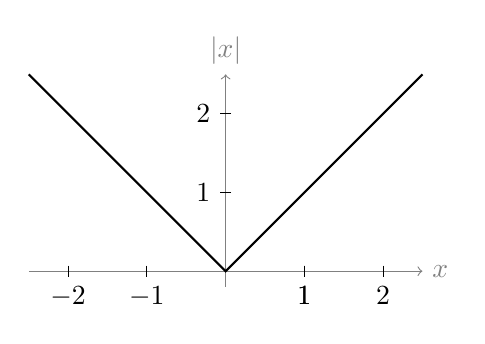
\begin{tikzpicture}[scale=1]
	\draw[->, gray] (-2.5,0) -- (2.5,0) node[right] {$x$};
	\draw[->, gray] (0,-.2) -- (0,2.5) node[above] {$|x|$};

	\foreach \x/\xtext in {-2/-2, -1,1, 1/1, 2/2}
	\draw[shift={(\x,0)}] (0pt,2pt) -- (0pt,-2pt) node[below] {{$\xtext$}};

	\foreach \y/\ytext in {1/1, 2/2}
	\draw[shift={(0,\y)}] (2pt,0pt) -- (-2pt,0pt) node[left] {{$\ytext$}};

	\draw[thick] (-2.5, 2.5)--(0,0)--(2.5, 2.5);
	\end{tikzpicture}
\end{center}
La définition dit donc, en première approximation, que l'on peut
rendre l'«~erreur~» inférieure à $\epsilon$ (c'est-à-dire obtenir
$|g(x) - \ell| < \epsilon$) en choisissant des arguments distincts
de~$c$ et situés à une distance inférieure à $\delta$ de~$c$
(c'est-à-dire tels que $0<|x-c|<\delta$).

Une fois la notion de limite définie, nous pouvons nous passer
entièrement des infinitésimaux et poser que la pente de $f$ au
point~$c$ est donnée par :
\[
	{f}'(c) = \lim_{x \rightarrow 0}\left(\frac{f(c +x) - f(c)}{x}\right)
	\text{ lorsque cette limite existe.}
\]
Il faut comprendre pourquoi cette définition doit comporter la
réserve «~lorsque cette limite existe~». Considérons l'exemple simple
de $f(x) = |x|$, dont nous venons de voir le graphe. Il est clair que
$f'(0)$ n'est pas définie : quand on s'approche de~$0$ «~par la
droite~», la pente vaut toujours~$1$ ; quand on s'en approche «~par
la gauche~», elle vaut toujours~$-1$. La limite n'existe donc pas.
Nous pouvons ainsi dire qu'une fonction~$f$ est \emph{dérivable}
en~$x$ si et seulement si une telle limite existe.

Nous avons vu comment traiter la dérivation à l'aide de la notion
de \emph{limite}. Celle-ci permet aussi de définir une fonction
\emph{continue}. Bolzano l'avait en substance compris dès 1817.
Voici l'approche de Cauchy et Weierstrass. Intuitivement, une
fonction~$f$ est continue en un point si toute précision exigée
pour sa valeur peut être garantie par une précision suffisante sur
son argument. Plus précisément, $f$ est continue en~$c$ lorsque,
si $x$ tend vers~$0$, la différence entre $f(c + x)$ et $f(c)$
tend elle aussi vers~$0$. Autrement dit, $f$ est \emph{continue}
en~$c$ si et seulement si
$f(c) = \lim_{x \rightarrow c} f(x)$.

Poursuivre nous entraînerait dans l'analyse réelle, alors que notre
sujet est la théorie des ensembles. Arrêtons-nous donc pour retenir
la leçon : au XIXe siècle, les mathématiciens apprirent à se passer
des infinitésimaux en recourant à une notion de \emph{limite}
définie rigoureusement.

\end{document}
